\section{Acceptors and Transducers}
\label{sec:acceptors_transducers}

\subsection{Automata}
\label{sec:automata}

The broad class of graphs we are going to look at are finite-state automata.
These include deterministic finite-state automata (DFAs) and non-deterministic
finite-state automata (NFAs). More specifically we will consider a
generalization of DFAs and NFAs called weighted finite-state acceptors (WFSAs).
That's a mouthful, so I will just call them \emph{acceptors}. We will also
consider a further generalization of an acceptor called a \emph{transducer}
(weighted finite-state transducers or WFSTs). Figure~\ref{fig:wfsa_classes}
shows the relation between these three graphs; transducers, acceptors, and
automata. Transducers are the most expressive in terms of their
representational power, followed by acceptors followed by unweighted automata.

\begin{figure}
    \centering
    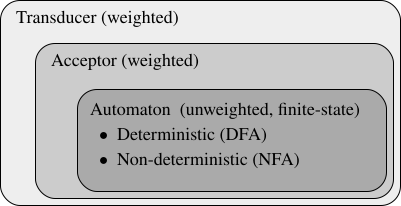
\includegraphics[width=0.7\linewidth]{figures/wfsa_classes}
    \caption{A hierarchy of automata classes from general to specific in terms
    of representation power. Weighted transducers can represent anything that
    weighted acceptors can represent. Weighted acceptors in turn can represent
    any unweighted finite-state automata.}
    \label{fig:wfsa_classes}
\end{figure}

Before we dive into acceptors and transducers, let's introduce some general
graph terminology that I will use throughout. In the following graph a
\emph{state} or \emph{node} is represented by a circle. The arrows represent
connections between two states. We usually refer to these as \emph{arcs} but
sometimes also \emph{edges}. The graph is directed since the connections
between states are unidirectional arrows. The arcs in a graph can have labels.
In Figure~\ref{fig:simple_automata} the arc between states $0$ and $1$ has a
label of $a$. Similarly, the arc between states $1$ and $2$ has a label of $b$.
The graph is an example of a finite-state automata (FSA) or finite-state
machine (FSM), so called because it has a finite number of nodes.

\begin{figure}
    \centering
    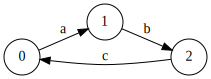
\includegraphics{figures/simple_automata}
    \caption{An example of a simple finite-state automata.}
    \label{fig:simple_automata}
 \end{figure}

An automata is deterministic if for each state and label pair there is only one
outgoing transition which matches that label. An automata is nondeterministic
if multiple transitions leaving a state have the same label. The graphs in
Figure~\ref{fig:dfa_nfa} show an example of a deterministic and a
nondeterministic automata. In general, acceptors and transducers can be
nondeterministic.

\begin{figure}
    \centering
    \begin{subfigure}[b]{0.48\textwidth}
        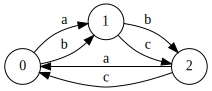
\includegraphics[scale=\dotscale]{figures/simple_dfa}
        \caption{Deterministic}
        \label{fig:simple_dfa}
    \end{subfigure}
    \begin{subfigure}[b]{0.48\textwidth}
        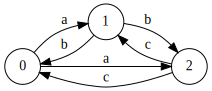
\includegraphics[scale=\dotscale]{figures/simple_nfa}
        \caption{Nondeterministic}
        \label{fig:simple_nfa}
    \end{subfigure}
    \caption{An example of a deterministic automata and a
    nondeterministic automata. The nondeterministic automata has
    two arcs leaving the state $2$ both with the label $c$.}
    \label{fig:dfa_nfa}
\end{figure}

\subsection{Acceptors}

Let's start by constructing some very basic automata to get a feel for their
various properties.

The start state $s = 0$ has a bold circle around it. The accepting state $1$ is
represented with concentric circles. Each arc has a label and a corresponding
weight. So the first arc from state $0$ to state $1$ with the text $a/0$ means
the label is $a$ and the weight is $0$. The fact that there is only a single
label on each arc means this graph is an \emph{acceptor}. Since it has weights,
we say its a weighted acceptor. Since the number of states is finite, some
would call it a weighted finite-state acceptor or WFSA. Again, that's a
mouthful, so I'll just call these graphs acceptors.

\begin{figure}
    \centering
    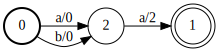
\includegraphics[scale=\dotscale]{figures/simple_fsa}
    \caption{An example of a simple acceptor. The label on each arc shows the
    input label and weight, so the $a/0$ represents a label of $a$ and a weight
    of $0$.}
    \label{fig:simple_fsa}
\end{figure}

An accepting path in the graph is a sequence of arcs which begin at a start
state and end in an accepting state. By concatenating the labels on an
accepting path, we get a string which is accepted by the graph. So the string
$aa$ is accepted by the graph by following the state sequence $0 \rightarrow 2
\rightarrow 1$. The string $ba$ is also accepted by the graph by following the
same state sequence but taking the arc with label $b$ when traversing from
state $0$ to state $1$. The language of the acceptor is the set of all strings
which are accepted by it. You may also encounter ``recognized'' used as a
synonym for ``accepted''. Let the variable $\gA$ represent the above acceptor.
In general, I'll use uppercase script letters to represent graphs. Let
$\mathcal{L}(\gA)$ denote the language of $\gA$. In this case $\mathcal{L}(\gA)
= \{aa, ba\}$.

There are different ways to compute the weight of a string accepted by the
graph. The most common is to sum the weights of the arcs on the accepting path
for that string. For example the string $aa$ in the above graph has a weight of
$0 + 2 = 2$. Another option would be to multiply the weights. These two options
correspond to interpreting the weights as either log probabilities or
probabilities. We'll have more to say about this later.

The graph in Figure~\ref{fig:multi_path} accepts the same sequence by multiple
paths.

\begin{figure}
    \centering
    \includegraphics[scale=\dotscale]{figures/multi_path}
    \caption{An acceptor which has multiple paths for the same sequence, $aa$.}
    \label{fig:multi_path}
\end{figure}

The string $aa$ is accepted along the state sequence $0 \rightarrow 2
\rightarrow 1$ and along the state sequence $0 \rightarrow 3 \rightarrow 1$. In
this case, to compute the score of $aa$ we need to consider both paths. Again
we have a couple of options here. The most common approach is to
\emph{log-sum-exp} the individual path scores. Again this corresponds to
interpreting the path scores as log probabilities. We'll use $\LSE(s_1, s_2)$
to denote the \emph{log-sum-exp} of the two scores $s_1$ and $s_2$:
\begin{equation}
\LSE(s_1, s_2) = \log \left( e^{s_1} + e^{s_2}\right).
\end{equation}
So the overall weight for the string $aa$ in the above graph is given by:
$$
\log \left(e^{0 + 2} + e^{1 + 3}\right) = 4.13.
$$

Acceptors can have multiple start states and multiple accept states. In the
graph in Figure~\ref{fig:multi_start_accept}, the states $0$ and $1$ are both
start states, and the states $3$ and $4$ are both accept states.

\begin{figure}
    \centering
    \includegraphics[scale=\dotscale]{figures/multi_start_accept}
    \caption{An acceptor with multiple start states ($0$ and $1$) and multiple
    accept states ($3$ and $4$).}
    \label{fig:multi_start_accept}
\end{figure}

It turns out that allowing multiple start or accept states does not increase
the expressive power of the graph. With $\epsilon$ transitions (which we will
discuss soon), one can convert any graph with multiple start states and
multiple accept states into an equivalent graph with a single start state and a
single accept state.

Note also that start states can have incoming arcs (as in state $1$) and accept
states can have outgoing arcs, as in state $3$.

\begin{example}
Compute the score of the string $ab$ in Figure~\ref{fig:multi_start_accept}.
\end{example}

\begin{proof}[\unskip\nopunct]
The two state sequences which accept the string $ab$ are the states $0
\rightarrow 2 \rightarrow 3$ and $1 \rightarrow 3 \rightarrow 4$. The overall
score is given by:
$$
\log (e^{1 + 3} + e^{1 + 2}) = 4.31.
$$
\end{proof}

Graphs can also have self-loops and cycles. For example, the graph in
Figure~\ref{fig:fsa_loops} has a self-loop on the state $0$ and a cycle
following the state sequence $0 \rightarrow 1 \rightarrow 2 \rightarrow 0$.

\begin{figure}
    \centering
    \includegraphics[scale=\dotscale]{figures/fsa_loops}
    \caption{A graph with a self-loop on the state $0$ and a cycle from $0
    \rightarrow 1 \rightarrow 2 \rightarrow 0$.}
    \label{fig:fsa_loops}
\end{figure}

The language of graphs with cycles and self-loops contain infinitely many
strings. For example the graph above accepts any string that starts with zero
or more $a$s and ends in $bb$. As a regular expression we write this as $a^*bb$
where the $^*$ denotes zero or more $a$s.

The $\epsilon$ symbols has a special meaning when it is the label on an arc.
Any arc with an $\epsilon$ label can be traversed without consuming an input
token in the string. So the graph in Figure~\ref{fig:fsa_epsilon} accepts the
string $ab$, but it also accepts the string $b$ because we can traverse from
state $0$ to state $1$ without consuming an input.

\begin{figure}
    \centering
    \includegraphics[scale=\dotscale]{figures/fsa_epsilon}
    \caption{An acceptor with an $\epsilon$ transition on the second arc
    between state $0$ and $1$.}
    \label{fig:fsa_epsilon}
\end{figure}

As it turns out, any graph with $\epsilon$-transitions can be converted to an
equivalent graph without $\epsilon$ transitions. However, this usually comes at
a large cost in the size of the graph. Complex languages can be represented by
much more compact graphs with the use of $\epsilon$-transitions.

\begin{example}
Convert the graph in Figure~\ref{fig:multi_start_accept} which has multiple
start and accept states to an equivalent graph with only a single start and
accept state using $\epsilon$ transitions.
\end{example}

\begin{proof}[\unskip\nopunct]
The graph in Figure~\ref{fig:epsilon_start_accept} is the equivalent graph
with a single start state and a single accept state.

\begin{figure}
    \centering
    \includegraphics[scale=\dotscale]{figures/epsilon_start_accept}
    \caption{The equivalent graph using only a single start state and accept
    state to the graph in figure~\ref{fig:multi_start_accept} which has
    multiple start and accept states.}
    \label{fig:epsilon_start_accept}
\end{figure}

The construction works by creating a new start state and connecting it to the
old start states with $\epsilon$ transitions with a weight of $0$. The old
start nodes are regular internal nodes in this new graph. Similarly the old
accept states are now regular states and they connect to the new accept state
with $\epsilon$ transitions with a weight of $0$.
\end{proof}

\subsection{Transducers}

A \emph{transducer} maps input strings to output strings. Transducers are a
generalization of an acceptors. Every acceptor is a transducer, but not every
transducer is an acceptor. Let's look at a few example transducers to
understand how they work.

The arc labels distinguish an acceptor from a transducer. A transducer has both
an input and output arc label. The arc labels are of the form $a\!:\!x/0$ where
$a$ is the input label $x$ is the output label and $0$ is the weight. An
acceptor can be represented as a transducer where the input and output labels
on every arc are identical.

\begin{figure}
    \centering
    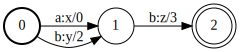
\includegraphics[scale=\dotscale]{figures/simple_fst}
    \caption{An example of a simple transducer. The label on each arc shows the
    input label, the output label, and the weight. So $a\!:\!x/0$ represents an
    input label of $a$, and output label of $x$, and a weight of $0$.}
    \label{fig:simple_fst}
\end{figure}

Instead of saying that a transducer accepts a given string, we say that it
\emph{transduces} one string to another. The graph in
Figure~\ref{fig:simple_fst} transduces the string $ab$ to the string $xz$ and
the string $bb$ to the string $yz$. The weights of a transduced pair is
computed in the same way as in an acceptor. The scores of the individual arcs
on the path are summed. The path scores are combined with \emph{log-sum-exp}.
So the weight of the transduced pair $(ab, xz)$ in the above graph is $0+3 =
3$.

We have to generalize concept of the language from an acceptor to a transducer.
I'll call this generalization the transduced set. Since it will always be clear
from context if the graph is an acceptor or transducer, I'll use the same
symbol $\mathcal{L}$ to represent the transduced set. If $\gT$ is a transducer,
then $\mathcal{L}(\gT)$ is the set of pairs of strings transduced by $\gT$.
More formally, a pair of strings $(\vx, \vy) \in \mathcal{L}(\gT)$ if $\gT$
transduces $\vx$ to $\vy$.

\begin{example}
Compute the score of the transduced pair $(aab, zyy)$ in the graph in
Figure~\ref{fig:fst_example_score}.
\end{example}

\begin{proof}[\unskip\nopunct]
\begin{figure}
    \centering
    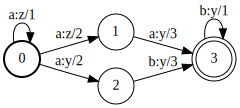
\includegraphics[scale=\dotscale]{figures/fst_example_score}
    \caption{An example transducer in which the sequence $aab$ is transduced to
    the sequence $zyy$ on multiple paths.}
    \label{fig:fst_example_score}
\end{figure}

The two paths which transduce $aab$ to $zyy$ are following the state sequence
$0 \rightarrow 1 \rightarrow 3 \rightarrow 3$ and $0 \rightarrow 0 \rightarrow
2 \rightarrow 3$. The score of the first path is $6$ and the score of the
second path is $6$. So the overall score is:
$$
\log \left(e^6 + e^6\right) = 6.69.
$$
\end{proof}

Transducers can also have $\epsilon$ transitions. The $\epsilon$ can be either
the input label on an arc, the output label on an arc, or both. When the
$\epsilon$ is the input label on an arc, it means we can traverse that arc
without consuming an input token, but we still output the arc's corresponding
output label. When the $\epsilon$ is the output label, the opposite is true.
The input is consumed but no output is produced. And when the $\epsilon$ is
both the input and the output label, the arc can be traversed without consuming
an input or producing an output.

\begin{figure}
    \centering
    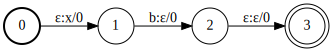
\includegraphics[scale=\dotscale]{figures/fst_epsilon}
    \caption{A transducer with $\epsilon$ transitions. The $\epsilon$ can be
    just the input label, just the output label, or both the input and output
    label.}
    \label{fig:fst_epsilon}
\end{figure}

In the graph in Figure~\ref{fig:fst_epsilon}, the string $b$ gets transduced to
the string $x$. On the first arc between states $0$ and $1$, we output an $x$
without consuming any token. On the second arc between states $1$ and $2$, a
$b$ is consumed without outputting any new token. Finally, on the arc between
states $2$ and $3$ we neither consume nor output a token.
